\documentclass[slides,compress]{beamer}
\usepackage{graphicx,amsmath,hyperref}
\usepackage{verbatim}

\usepackage[normalem]{ulem}

\usetheme{default}
\useinnertheme{rectangles}

\title{\huge Novel Uses for \emph{xia2} in a Beamline Environment}
\subtitle{\large Harvard Medical School, July 2012}

\author{Graeme Winter}
\institute{Diamond Light Source}
\date{July 2012}

\begin{document}

\setbeamertemplate{background}{

\includegraphics[width=\paperwidth,height=\paperheight]
{diamond-background.png}
}

\frame{\maketitle}

\frame{
\frametitle{Overview}
\begin{itemize}
\item{Context}
\item{At Diamond Light Source}
\item{Options for lower level interaction}
\item{How does this help?}
\end{itemize}
}

\frame{
\frametitle{Acknowledgements}
\begin{itemize}
\item{Thanks to Nick Sauter for suggesting this - moving in an
    interesting direction}
\item{\emph{xia2} funded through BBSRC e-Science e-HTPX project, CCP4,
    BioXHit and Diamond Light Source}
\item{Users, providers of test data, lots of people who have provided
    input into project, Diamond Light Source staff}
\end{itemize}
}

\frame{
\frametitle{Context / Background}
\begin{itemize}
\item{\emph{xia2} initially developed as part of e-HTPX project,
    supported by CCP4 and EU, now Diamond Light Source}
\item{Started work on DNA project in 2002 - kept this in mind}
\item{Original thoughts behind xia2 were to cover scope from data
    collection through reduction to phasing / refinement}
\item{Implemented middle bit}
\item{\emph{xia2} is properly free open source software}
\item{\emph{xia2} possible conduit for delivering DIALS software to
    beamlines}
\end{itemize}
}

\frame{
\frametitle{\emph{xia2} at Diamond Light Source}
\begin{itemize}
\item{Full functionality available to users manually}
\item{Run automatically (has been so for five years or so) on a
    per-sweep basis - xia2 -blah -image /path/to/an/image}
\item{Automatic running essentially fire and forget - results
    available to user, not integrated into data collection system}
\item{Rather than providing fine grained user control, run several
    jobs}
\item{Inspired development of fast DP - a very much cut down
    ``script'' for performing simple data analysis with XDS, in very
    short time}
\end{itemize}
}

\frame{
\frametitle{Fast DP}
Fast processing with Fast DP - script which runs XDS on up to 480 cpus
to deliver data reduction (frames to merged MTZ, merging stats) in
under 2 minutes, even for 1800 frame Pilatus sets.
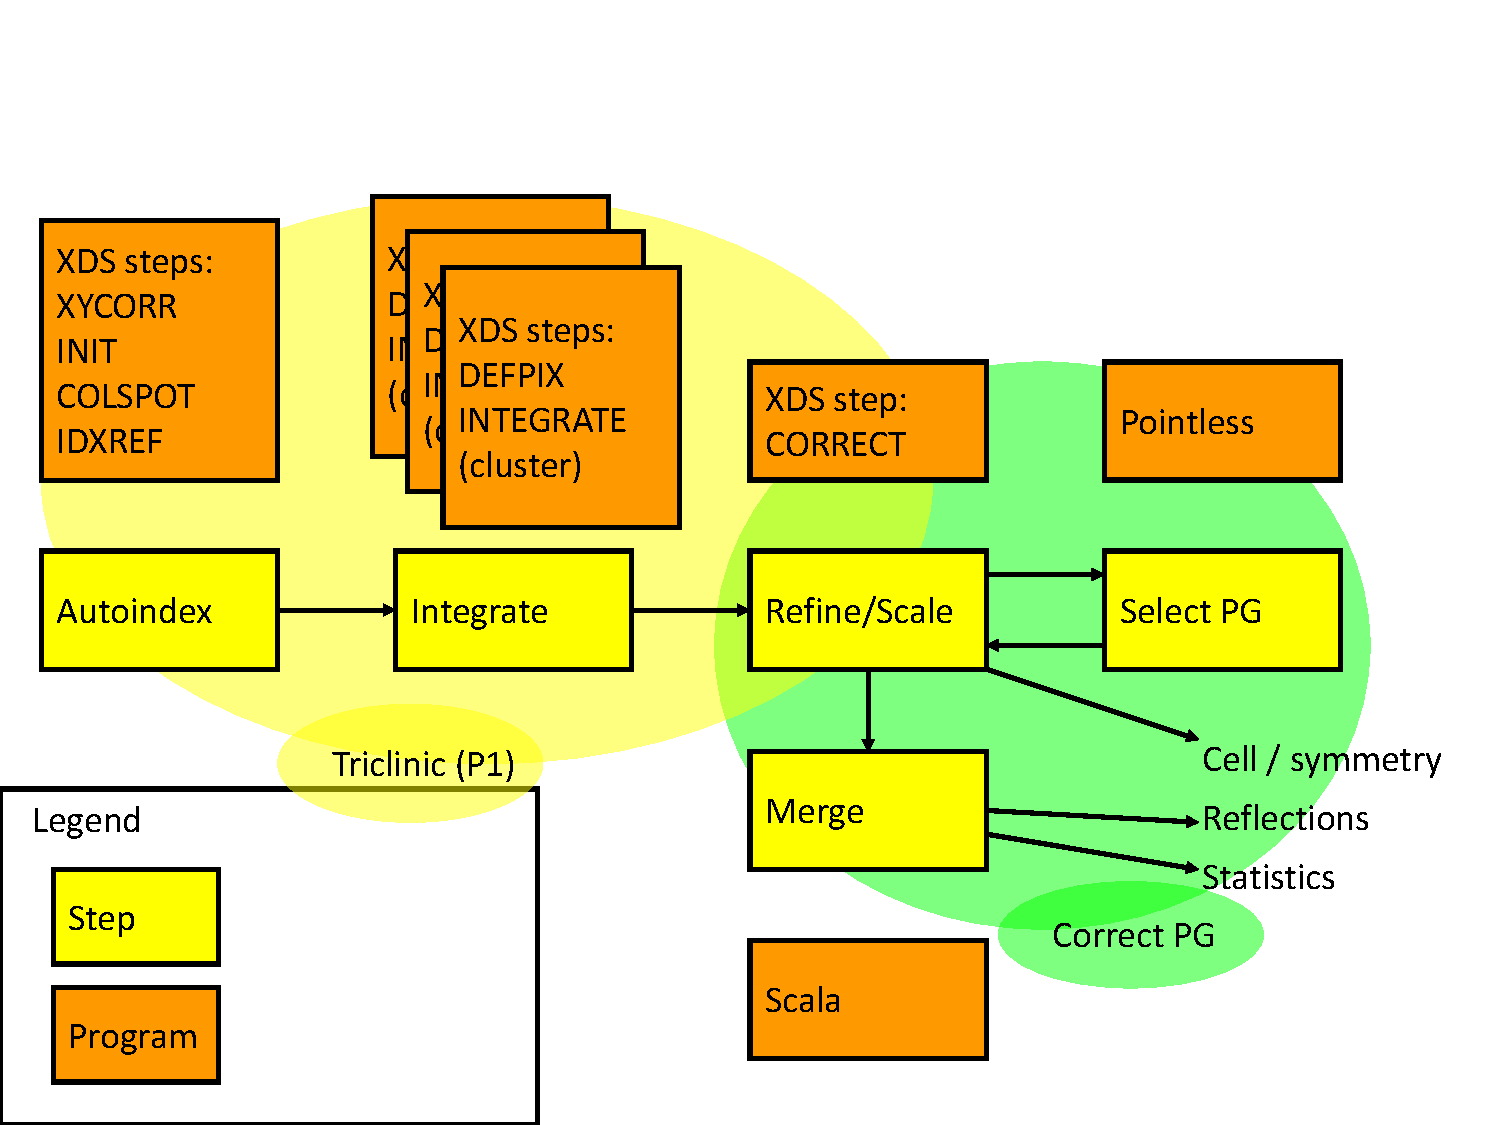
\includegraphics[scale=0.4]{fast-dp-diagram.pdf}
}

\frame{
\frametitle{Dimple}
Following Fast DP - compute difference map from known native
structure, particularly useful for industry. Map available within a
few minutes of the experiment.
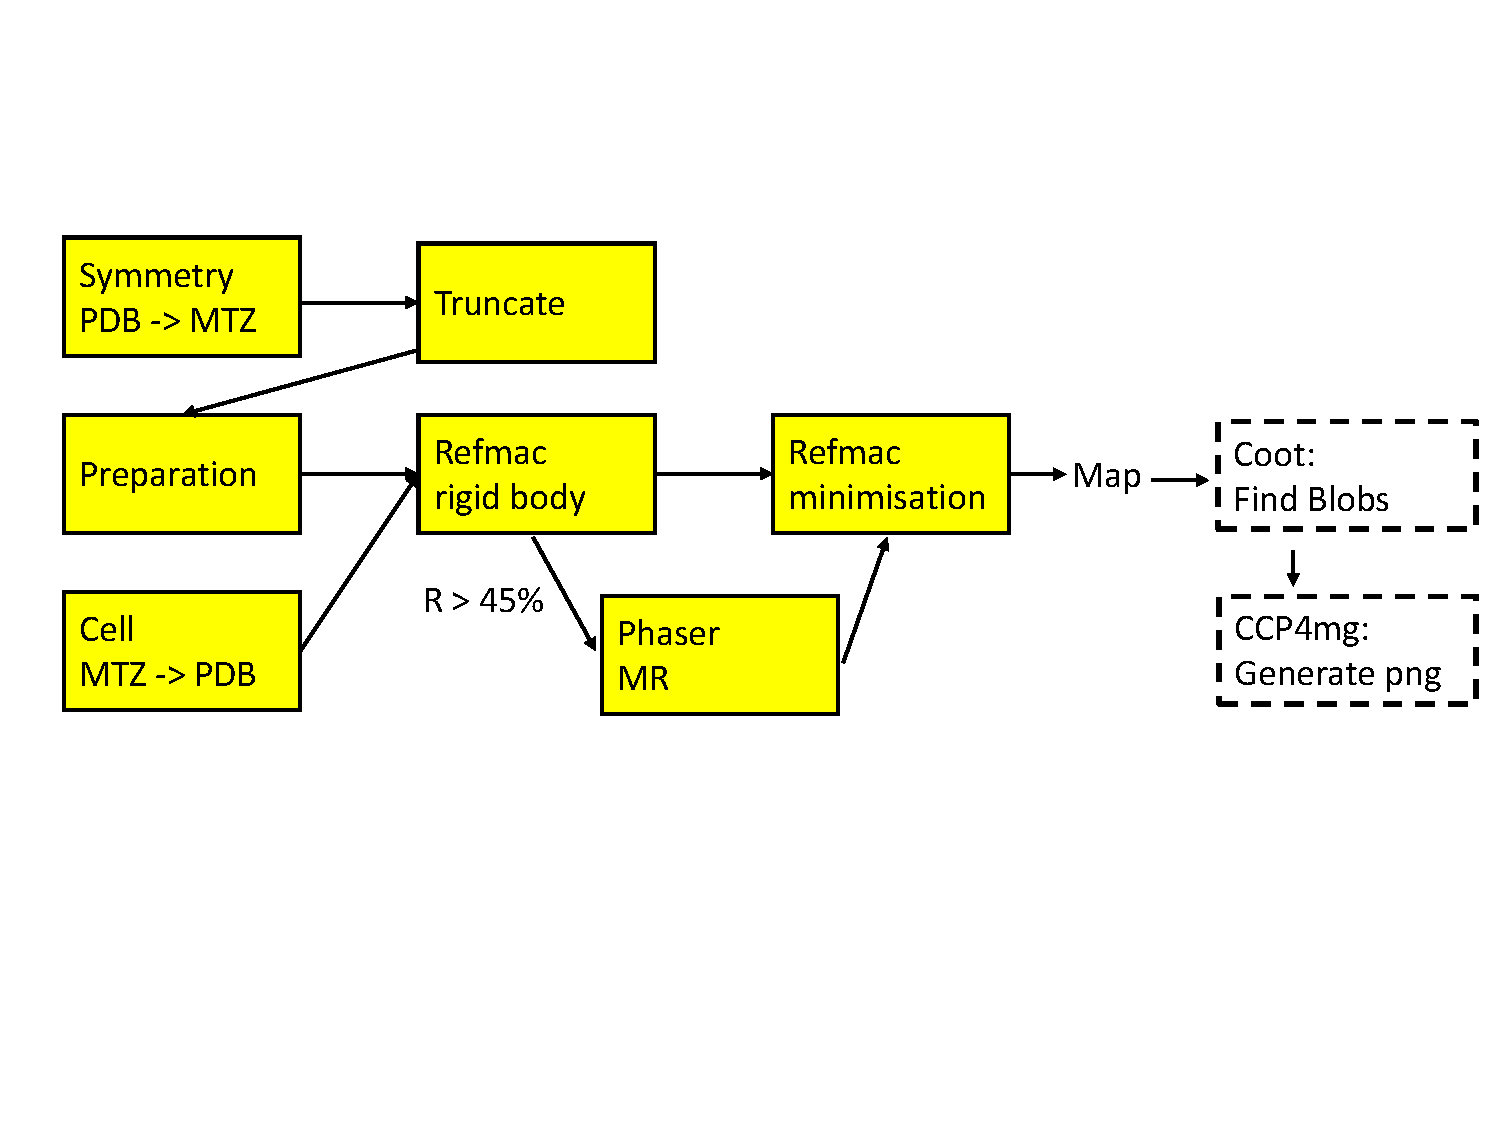
\includegraphics[scale=0.4]{dimple-diagram.pdf}
}

\frame{
\frametitle{Per-image analysis}
Run DISTL on every image / 250 from wedge, plot - gives near real-time
feedback on diffraction. Useful for characterising what happened to sample.
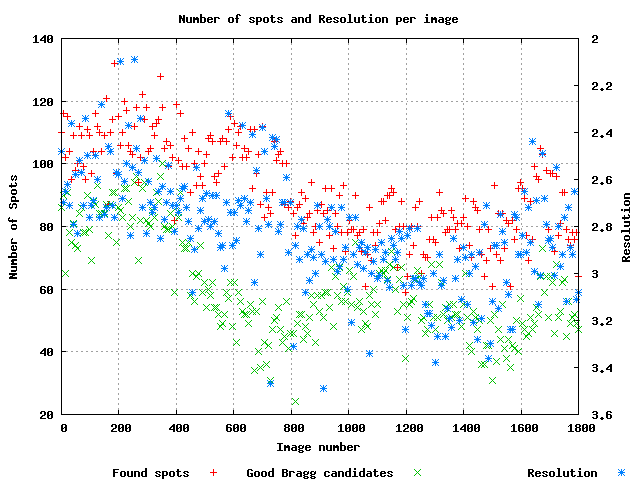
\includegraphics[scale=0.4]{pia.png}
}

\frame{
\frametitle{Benefits with this approach}
\begin{itemize}
\item{Lack of user interaction - they can get on with data collection}
\item{Now considered by users a beamline component - they complain on
    feedback forms when it fails}
\item{All data is processed during the beam time  - users can plan
    experiments properly}
\end{itemize}
}

\frame{
\frametitle{Issues with this approach}
\begin{itemize}
\item{Lack of user interaction}
\item{Timescale, hence Fast DP (next slide)}
\item{Per-sweep \emph{xia2} problem: does not sit nicely with
    e.g. MAD, multi-sweep data collection}
\item{Feedback to user is not assertive i.e. direct feedback to data
    collection system}
\item{\emph{Does not handle incremental feedback well}}
\end{itemize}
}

\frame{
\frametitle{Lower-level interaction with \emph{xia2}}
\begin{itemize}
\item{Main \emph{xia2} program is a print statement (really) - all
    processing performed to deliver the results of this print
    statement}
\item{However, the code is \emph{just Python}}
\item{Let's look at a lower level interaction}
\end{itemize}
}

\begin{frame}[fragile]
\tiny{
\begin{verbatim}
    from Handlers.PipelineSelection import add_preference
    directory, image = os.path.split(sys.argv[1])

    from XProject import XProject
    from XCrystal import XCrystal
    from XWavelength import XWavelength
   
    xp = XProject(name = 'example')
    xc = XCrystal('demonstration', xp)
    xw = XWavelength('native', xc)
    xw.add_sweep('native', directory, image)
   
    print 'Scaled data: %s' % xc.get_scaled_merged_reflections()['mtz']
\end{verbatim}
}
\end{frame}

\frame{
\frametitle{Observations}
\begin{itemize}
\item{Code above will work}
\item{It will also write a lot of junk to stdout}
\item{May also generate extra directories - full fat version next slide}
\end{itemize}
}

\begin{frame}[fragile]
\tiny{
\begin{verbatim}
    from Handlers.PipelineSelection import add_preference
    from Handlers.Streams import streams_off
    from Handlers.Environment import Environment

    Environment.dont_setup()
    streams_off()

    add_preference('indexer', 'labelit')
    add_preference('integrater', 'xdsr')
    add_preference('scaler', 'xdsr')

    directory, image = os.path.split(sys.argv[1])

    from XProject import XProject
    from XCrystal import XCrystal
    from XWavelength import XWavelength
   
    xp = XProject(name = 'example')
    xc = XCrystal('demonstration', xp)
    xw = XWavelength('native', xc)
    xw.add_sweep('native', directory, image)
   
    print 'Scaled data: %s' % xc.get_scaled_merged_reflections()['mtz']
\end{verbatim}
}
\end{frame}

\frame{
\frametitle{Moving on}
\begin{itemize}
\item{This code will \emph{silently} process your data, scale and
    return a merged MTZ file containing intensities and amplitudes}
\item{Provided handle to xp or xc kept can interrogate nearly everything}
\item{\emph{Aha!} why can't I just add another sweep and get
    reflections again? Bugs}
\item{Code was never written to work like this, though with a couple
    of hours work could be}
\item{Move control of system from command-line input to Phil objects -
    more easily embedded}
\end{itemize}
}

\frame{
\frametitle{How does this help?}
\begin{itemize}
\item{Lower level access to \emph{xia2} machinery}
\item{More control from caller pespective}
\item{Capability to provide user interface - user can (in principle)
    add and remove sweeps, tweak processing on live system}
\item{Capability for system to keep adding sweeps (say multi-crystal
    environment) until complete data set achieved}
\end{itemize}
}

\frame{
\frametitle{What needs doing?}
\begin{itemize}
\item{Mainly resolving dependencies in the analysis - xia2 is dynamic
    enough already
\begin{itemize}
\item{e.g. when sweep added to wavelength, scaling needs repeating}
\item{e.g. when images added to a sweep integration needs repeating}
\end{itemize}
}
\item{Probably a couple of days work - not hours, I tried the other day}
\item{Testing - this is an approach which has never been tested inside
    xia2 though should work}
\end{itemize}
}

%\frame{
%\frametitle{Next steps: DIALS}
%\begin{itemize}
%\item{Project part of Biostruct-X EU FP7 project, funded by EU,
%    Diamond Light Source and CCP4, collaborating with New Horizons}
%\item{Aim to develop new integration framework and algorithms - next
%    talk}
%\item{Aim to provide interface \emph{via} \emph{xia2}}
%\end{itemize}
%}

\end{document}
